\chapter{\K{}-based Computer Interpretable Guidelines}

In \autoref{chapter:separating-concerns}, we described an
architecture for building safe and modular clinical decision support systems.
We split \CDSSs{} into three separate components:
\begin{enumerate*}[label=(\alph*)]
  \item a frontend that facilitates interaction with \HCPs{},
  \item a backend that serves as a computer-interpretable encoding of the \BPG{}, and,
  \item additional infrastructure that wires components together.
\end{enumerate*}
This, and upcoming chapters, focus on building backends for \CDSSs{}
utilizing the \emph{semantics-first} approach described in
\autoref{chapter:semantics-first-cdss}. By semantics-first, we
mean that:
\begin{enumerate*}[label=(\alph*)]
 \item the semantics of medical knowledge in the \BPG{} is
 accurately captured, and,
 \item the semantics of the language used to describe the
 \BPG{} is formally defined.
\end{enumerate*}

In \autoref{sec:generic-bpg}, we briefly described characteristics
of \BPGs{} that a \CIG{} language must accommodate.
To this end, we attempted to come up with a framework that
can accommodate expressing a large number of diverse \BPGs{}.
Thus, we broke \BPGs{} into smaller statements that we organized
into:
\begin{itemize}
  \item a workflow containing statements that are executed sequentially, and,
  \item workflows within a guideline may be executed concurrently.
\end{itemize}

In this chapter, we describe a methodology to encode real-world \BPGs{}
as $\K$ definitions. Execution in $\K{}$ is inherently concurrent---
if more than one $\K{}$ rule can apply, then $\K$ non-deterministically
chooses one. Thus, we describe a way of systematically encoding
medical knowledge in \BPGs{} as $\K$ definitions. First, in
\autoref{sec:acls}, we utilize a real world \BPG{} to come up
with an abstract representation that captures the \BPGs{}'s semantics
with enough details to enable computer-interpretation.
Next, \autoref{sec:bpg-in-k} describes translating said abstract representation
to a concrete, computer-interpretable format as a $\K{}$ definition.
Finally,

\section{Advanced Cardiovascular Life Support Guidelines (\ACLS{})}\label{sec:acls}

\begin{figure}[t!]
  \centering
  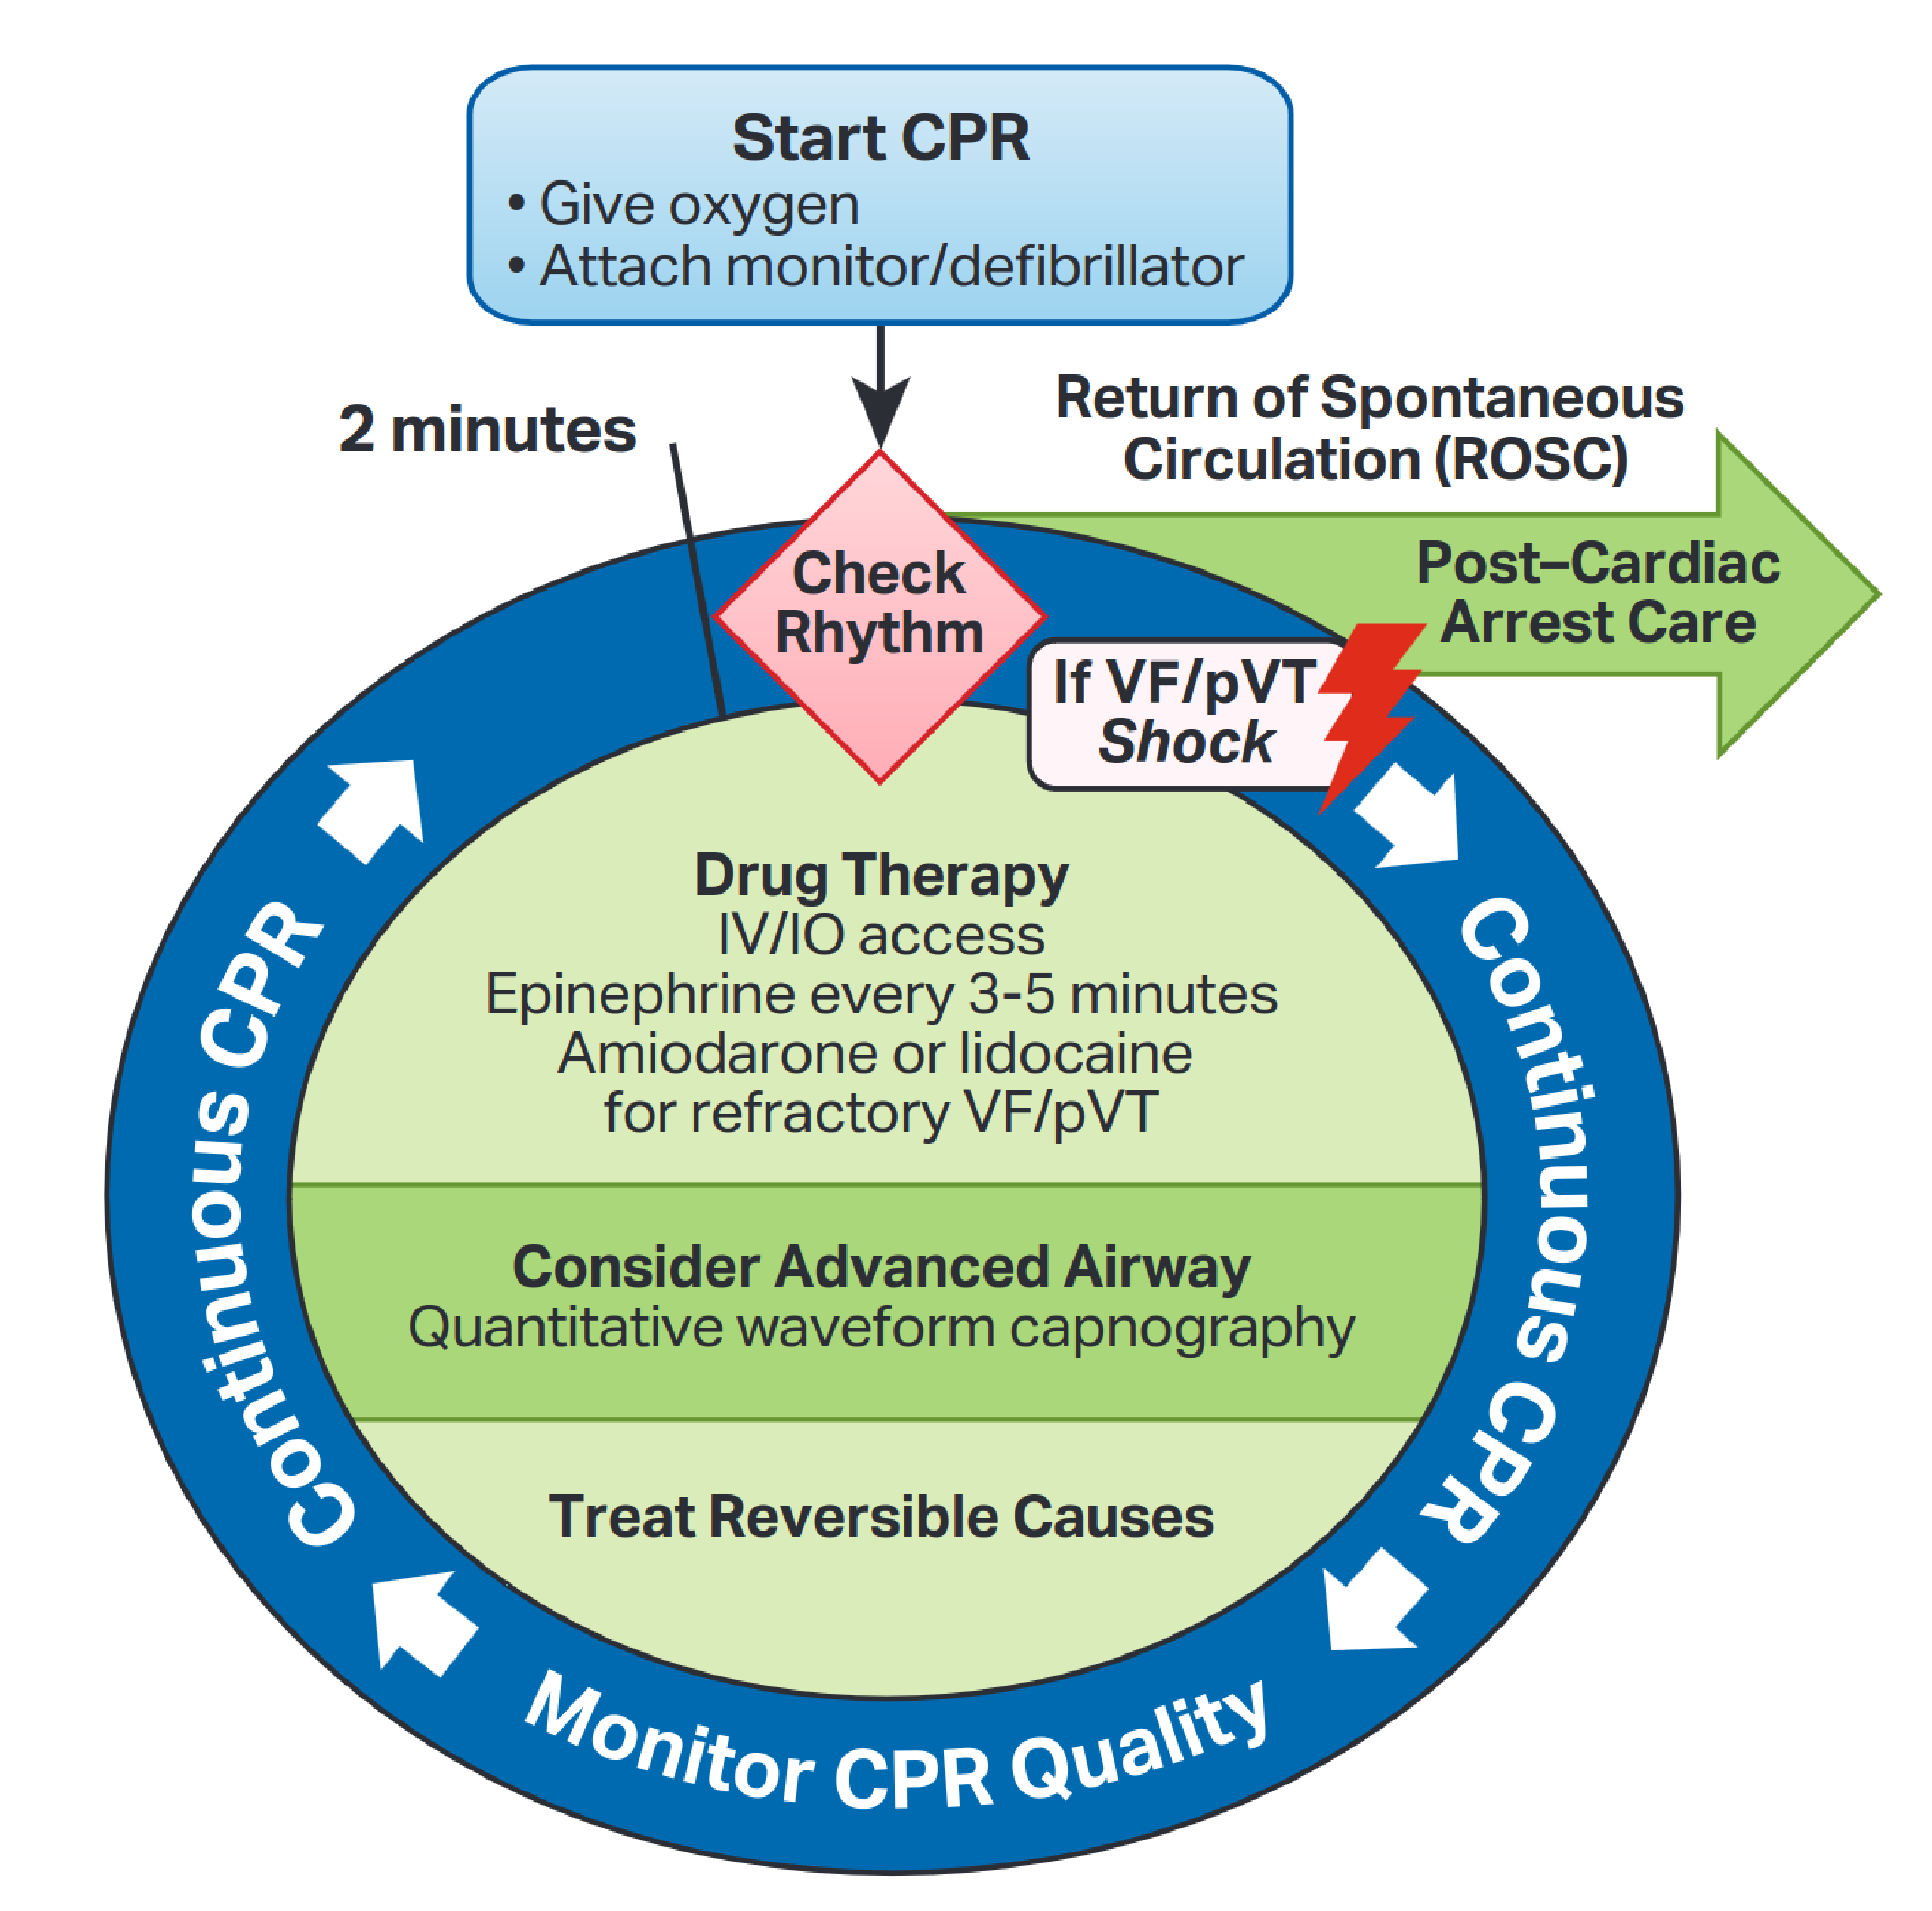
\includegraphics[width=0.8\textwidth]{acls-algorithm}
  \caption{Advanced Cardiac Life Support Guidelines}\label{fig:acls-algorithm}
\end{figure}

Advanced Cardiovascular Life Support (\ACLS{}) are a set of \BPGs{} periodically
published by the American Heart Association (\AHA{}) for management of
life-threatening cardiac conditions that will cause of have caused cardiac
arrest---a cardiac emergency where the heart stop pumping \cite{ACLSWikiEntry}.
The guidelines, according to the AHA{}, \say{are based on the most current
and comprehensive review of resuscitation science, systems, protocols, and
education} \cite{ACLSUrl}.

\autoref{fig:acls-algorithm} shows the \AHA{}'s guidelines for advanced
life support (\ALS{}) for adults \cite{ACLSGuidelineUrl}.
\AHA{} also publishes guidelines
for basic life support (\BLS{}), and pediatric counterparts of both. While
\BLS{} is meant for a first responder to provide treatment with
limited resources, such as an automatic emergency defibrillator (\AED{}),
\ACLS{} is supposed to be followed by teams of
trained professionals with advanced equipment for airway management,
drug delivery, etc. Cardiac arrest is an urgent condition that requires
prompt treatment. Immediate \ACLS{} guidelines-conformant has been
shown to improve patient outcomes \cite{HonarmandResuscitation18}.
Moreover, deviations from the guidelines in in-hospital cases has been
associated with decreased rates of return of spontaneous circulation (\ROSC{}),
 survival to discharge, and survival to discharge with favorable neurological
 outcomes \cite{CrawleyResuscitation20}.




The guidelines require an electrocardiography (EKG) machine
to monitor the patient's \textit{cardiac rhythm}, which can be
\textit{shockable} or \textit{unshockable}.
In case of a \textit{shockable
rhythm}, a \textit{defibrillator} device can be used to administer
a therapeutic electric shock. Furthermore, \textit{Cardiopulmonary Resuscitation} (CPR),
and drugs such as \textit{Epinephrine} must be periodically administered.
The algorithms is succinctly presented in figure \ref{fig:acls-algorithm} taken
from the AHA's ACLS documentation \cite{AHAUrl}


\section{Encoding Medical Guidelines as $\K$ Definitions}\label{sec:bpg-in-k}


